\documentclass[12pt,a4paper]{report}     % font size= 12,paper size= a4, document type= report 
\usepackage{graphics}
\usepackage[font=small,labelfont=bf]{caption}
\usepackage{fancybox}		% For formatting of cover page5
\usepackage{amsmath}    	% For  mathematical formulae
\usepackage{amssymb}
\usepackage{setspace}		% For adjusting line spacing 
\usepackage{pdfpages}
\usepackage{hyperref}                     % pacakage for 
\usepackage{fancyhdr}                     % pacakage for including header and footer 
\usepackage{times}                        % package for font type
\usepackage[left=1in,right=1in,top=1in,bottom=0.8in]{geometry} %
\usepackage{url}
\usepackage{rotating}
\usepackage{array}
\usepackage{enumitem}
%\usepackage{bbding}
\usepackage{amsfonts}
\usepackage{pythonhighlight}

\makeatletter
\def\@makechapterhead#1{%
  \vspace*{5\p@}%
  {\parindent \z@ \raggedright \normalfont
    \ifnum \c@secnumdepth >\m@ne
       \LARGE\bfseries \space \thechapter. \space
    \interlinepenalty\@M
    \LARGE \bfseries #1\par\nobreak
    \vskip 10\p@
  }}
  \makeatother
\begin{document}
\newpage
\pagestyle{plain}
\pagestyle{empty}
\pagestyle{fancy}							%display header, footer
\renewcommand{\headrulewidth}{0pt}
%\pagenumbering{arabic}						%display page numbers in arabic								 %set header to left	

\fancyfoot[LO]{\textit{P:F-SMR-UG/08/R0}}			%set footer to left
\fancypagestyle{plain}{}

 %\thispagestyle{empty}
	\pagenumbering{gobble}
	\thisfancyput(-0.0in,-10.0in){%
	%\thisfancypage{%
%\setlength{\fboxrule}{1pt}\doublebox}{} 
\setlength{\unitlength}{1in}\framebox(6.7,10.2)}
\begin{center}
      
      \begin{center} {A} \end{center}
      \vspace{0.2 in}
      { SEMINAR REPORT}
      \vspace{0.2 in}\\
       ON
			\end{center}
	\begin{center}
	    \vspace{0.1 in}
		\-\hspace{0.5cm}\textbf{\large  NATURAL LANGUAGE PROCESSING IN CHATBOT TECHNOLOGY  } % Give Your Seminar Title
		\vspace{0.2 in}
	\end{center}
     \vspace{0.2 in}
		\begin{center}
	    SUBMITTED TO THE SAVITRIBAI PHULE PUNE UNIVERSITY, PUNE \\
	    IN PARTIAL FULFILLMENT OF THE REQUIREMENTS\\
	    FOR THE AWARD OF THE DEGREE OF
	\end{center}
	\vspace{0.1 in}
	
	\begin{center}
	   {BACHELOR OF ENGINEERING}\\
	    \begin{small}{ INFORMATION TECHNOLOGY}
\end{small}	\end{center}
	\vspace{0.1 in}
	
	\begin{center}
	   \textbf{BY}
	\end{center}
	\vspace{0.1 in}
	
	\begin{center}
	   Pranish Warke\\ % instead of this word "Name" write your name"
	   \  Roll No: 33381 \\    % write roll No. instead of XXXXX
	   \ Exam Seat No:  \  \vspace{0.2 in}           %Write Exam Seat No. instead of XXX
	\end{center}
	\vspace{0.1 in}
	
	\begin{center}
	    {Under the guidance of }\\
	    {Mr.Sachin D. Shelke}  % Here write Your Seminar Guide Name
	\end{center}

		\vspace{0.1in}

	\begin{center}
	  \begin{figure}[h]
			\centering
			
\includegraphics[width=5cm]{pict_logo.png}
		\end{figure}
		\vspace{0.1cm}
	  \begin{large}\textsc {Department Of Information Technology} \end{large}\\
	  \textsc{Pune Institute of Computer Technology}\\
	  \textsc{Sr. No 27, Pune-Satara Road, Dhankawadi}\\
	  \textsc{Pune - 411 043.}\\
	      AY: 2022-2023
	\end{center}

%------------------------------------------------------------------------------
%  Cover ends here
%------------------------------------------------------------------------------
%------------------------------------------------------------------------------
%  Certificate starts here
%------------------------------------------------------------------------------
\newpage
\pagestyle{plain}
\pagestyle{empty}
\pagestyle{fancy}							%display header, footer
\renewcommand{\headrulewidth}{0pt}
%\pagenumbering{arabic}						%display page numbers in arabic								 %set header to left	
\fancyfoot[LO]{\textit{P:F-SMR-UG/08/R0}}			%set footer to left
\fancypagestyle{plain}{}

 %\thispagestyle{empty}
		\pagenumbering{roman}
		
	\thisfancyput(-0.15in,-9.7in){%
	%\thisfancypage{%
%\setlength{\fboxrule}{1pt}\doublebox}{} 
\setlength{\unitlength}{1in}\framebox(6.7,10.2)}
\begin{center}

{ SCTR's
   PUNE INSTITUTE OF COMPUTER TECHNOLOGY \\
   \small{DEPARTMENT OF INFORMATION TECHNOLOGY} \\

}
\vspace{0.2in}

\vspace{0.2in}

\includegraphics[width=5cm]{pict_logo.png}
\end{center}
\vspace{0.4in}
\begin{center}
\textbf{\underline{C E R T I F I C A T E}}
\vspace{0.2in}
\end{center}
		\noindent
  				\setlength{\baselineskip}{1.1\baselineskip}
	\begin{center}
This is to certify that the Seminar work entitled \\
		{NATURAL LANGUAGE PROCESSING IN CHATBOT TECHNOLOGY } 
%\singlespace
\begin{center} {Submitted by }\end{center}

Name : Pranish Warke\\   %Wrie Name in the place of XXXXXXXXXXX
Exam Seat No:\hspace{0.4in}.%Wrie Exam seat no.in the place of  XXXXXXXXXXX
	\end{center}
\onehalfspace
\begin{quote}
is a bonafide work carried out under the supervision of   {Name of the  Seminar Guide}  and it is submitted towards the partial fulfillment of the requirements of Savitribai Phule Pune University, Pune for the award of the degree of Bachelor of Engineering (Information Technology).
\end{quote}
		\noindent 
		\vspace{0.2 in}
\begin{quote}
\singlespace
%\\[0.5in]
{Mr.Sachin D. Shelke} % include Seminar Guide Name
\hspace{2.8in} Dr. A. S. Ghotkar\\
Seminar Guide\hspace{3.5 in}       HOD IT \\\\\\
\begin{center}  Dr. S. T. Gandhe   \\
  Principal 
 \end{center}


Date: 07/11/2022      \\ %write date in the form of dd/mm/yyyy format
Place: Pune      %write place as Pune
\\\\


 \end{quote}
\addcontentsline{toc}{section}{Certificate}
%------------------------------------------------------------------------------
%  Certificate ends here
%------------------------------------------------------------------------------

\newpage	
\pagestyle{plain}
%\pagestyle{empty}
\pagestyle{fancy}							%display header, footer
\renewcommand{\headrulewidth}{0pt}
%\pagenumbering{arabic}						%display page numbers in arabic								 %set header to left	
\fancyfoot[LO]{\textit{}}			%set footer to left
\fancypagestyle{plain}{}%start a new page
		\pagestyle{plain}           %dont display header footer and page nos
%\vline
		\begin{center}				%centre align the text
			\begin{LARGE}
	\section*{Acknowledgement}
			\addcontentsline{toc}{section}{Acknowledgement}
				%leave space of 0.5 inches vertically
			\end{LARGE}
		\end{center}
		\begin{normalsize}
%				\begin{quote}
{\setlength{\baselineskip}{1.1\baselineskip}
\noindent %Start acknowledgement from here.
Purpose of acknowledgments page is to show appreciation to those who contributed in
conducting this dissertation work / other tasks and duties related to the report writing. Therefore when writing acknowledgments page you should carefully consider everyone who helped during research process and show appreciation in the order of relevance. In this regard it is suitable to show appreciation in brief manner instead of using strong emotional phrases. 
\newline
In this part of your work it is normal to use personal pronouns like “I, my, me” while in the rest of the report this articulation is not recommended. Even when acknowledging family members and friends make sure of using the wording of a relatively formal register. The list of the persons you should acknowledged, includes guide (main and second), head of dept, academic staff in your department, technical staff, reviewers, head of institute, companies, family and friends. 
\newline
You should acknowledge all sources of funding. It’s usually specific naming the person and the type of help you received. For example, an advisor who helped you conceptualize the seminar,someone who helped with the actual building or procedures used to complete the seminar,someone who helped with computer knowledge, someone who provided raw materials for the seminar, etc.








			\vspace{1.8in}
				\begin{flushright} 
				Name : Pranish Warke\\ % Write Your Name in place of XXXXXX
			    Exam Seat No: \hspace{0.1in} %Write Exam seat No. in the place o %fXXX
				\end{flushright}
%				\end{quote}

}
		\end{normalsize}
		
%-----------------------------------Abstract------------------------------------------
		\newpage					%start a new page
		\pagestyle{plain}           %dont display header footer and display page nos
		\begin{center}				%centre align the text
			\begin{LARGE}
						\section*{ Abstract}
			%\vspace{.15 in}       %leave space of 0.5 inches vertically
			\end{LARGE}
		\end{center}
		\begin{normalsize}
{\setlength{\baselineskip}{1.1\baselineskip}   %set line spacing as 1.5
\noindent % Start writing abstract from here.
Chatbot Technology using natural language processing is a computer program, which responds like a smart entity when conversed with through text or voice and understands one or more human languages by Natural Language Processing (NLP). Basically, a chatbot is defined as “A computer program designed to simulate conversation with human users, especially over the Internet”. Artificial intelligence (AI), natural language processing (NLP), and machine learning are chatbot underlying technologies. To make the message understandable for a chatbot, NLP follows main techniques : Semantic analysis and neural machine translation. Chatbots are also known as smart bots, interactive agents, digital assistants, or artificial conversation entities. Chatbots are capable of constant and automated refinement. Smart bots are used in spam detection, chatbots are used as digital assistants by Google, Amazon, etc. Chatbots are used to enhance customer experience by various healthcare and e-commerce websites. Customer service chatbots provide value to customers as well as businesses. \\\\ 
\textbf{Keywords:} % start writing Keywords from here
Natural Language Processing, Machine Learning, Artificial Intelligence,
neural networks, NLU, deep learning\\\\
\par}
		\end{normalsize}
\addcontentsline{toc}{section}{Abstract}
%---------------------------------Abstract ends---------------------------------------
\newpage

\thispagestyle{empty}
\fancyhead{}
\renewcommand{\headrulewidth}{0pt}
%\fancypagestyle{plain}{}%start a new page
%		\thispagestyle{plain} 

\addcontentsline{toc}{section}{Contents}
\tableofcontents	 								% auto generate table of contents
\newpage
{\setlength{\baselineskip}{1.1\baselineskip}        % auto generate list of figures  
\listoffigures
\addcontentsline{toc}{section}{List of Figures}   % add to table of contents
}
\newpage
{\setlength{\baselineskip}{1.1\baselineskip}        % auto generate list of tables   
\listoftables
\addcontentsline{toc}{section}{List of Tables}
}
%---------------------------Abbrevations------------------------------------------------------------
\newpage
		\begin{LARGE}
			\begin{flushleft}
				\section*{\centering{Abbreviations}}
			\end{flushleft}
		\end{LARGE}
		\addcontentsline{toc}{section}{Abbreviations}	
\begin{normalsize}
					\noindent
{\setlength{\baselineskip}{1.1\baselineskip}
\vspace{0.2 in}
\begin{tabular}{lll}
\vspace{0.1 in}
NLP	&	:	&	Natural Language Processing	\\
\vspace{0.1 in}
AI	&	:	&	Artificial Intelligence 	\\
\vspace{0.1 in}
LSTM	&	:	&	Long Short Term Memory 	\\
\vspace{0.1 in}
GRU	&	:	&	Gated Recurrent Unit 	\\
\vspace{0.1 in}
RNN	&	:	&	Recurrent Neural Networks 	\\
\vspace{0.1 in}
DNN	&	:	&	Deep Neural Networks 	\\
\vspace{0.1 in}
CNN	&	:	&	Convolutional Neural Networks	\\
\vspace{0.1 in}
GUI	&	:	&	Graphical User Interface	\\
\vspace{0.1 in}
ML	&	:	&	Machine Learning	\\
\end{tabular}
\par}
\end{normalsize}

%-----------------------------------Chapter 1 Introduction}
\newpage
%\clearpage
\pagestyle{fancy}							%display header, footer
\pagenumbering{arabic}	%display page numbers in arabic
\renewcommand{\headrulewidth}{0.5pt}
\fancyhead[RO]{\textit{NLP in Chatbots }} %set header to right
\fancyhead[LO]{\textit{Seminar Report}}												 %set header to left	
\renewcommand{\footrulewidth}{0.5pt}		% print horizontal line in the footer of 0.5 pt
\fancyfoot[RO]{\textit{Dept. of Information Technology}}		%set footer to right
\fancyfoot[LO]{\textit{PICT,Pune}}			%set footer to left
\fancypagestyle{plain}{}
\pagenumbering{arabic}	
\chapter{\centering{Introduction}}
\begin{normalsize}
			\noindent

%-------------------------------------------------------------------------------------------------------
%  Start writing from here.
%(short para about your area describing its place in the world of Technology)
\section{Introduction} 	
{\setlength{\baselineskip}{1.1\baselineskip}
Natural Language Processing is a field in Artificial Intelligence where computer understands the human languages like English, Marathi, Hindi etc. Chatbot is an application of Natural Language Processing where user can chat with the computer like a user would have otherwise done with a human.  
\par
}	
\section{Motivation}
{\setlength{\baselineskip}{1.1\baselineskip}
%Start writing from here.
Nowadays, Chatbot technology is widely used by various organizations over the Internet to provide support and service to their customers. Using Natural Language Processing, we can improve the interaction between user and chatbots by using spoken language for communication.
\par}	

\section{Objectives}
{\setlength{\baselineskip}{1.1\baselineskip}
%Start writing from here.
Studying the implementation of natural language processing and neural networks in AI-powered chatbot technology.

\section {Scope}
{\setlength{\baselineskip}{1.1\baselineskip}
%Start writing from here.
Scope consists of study of general purpose in-app support chatbots that provide 24/7 customer service and text-to-text conversation using natural language processing.


%-----------------------Literature Survey & Discussion (Literature Survey)----------------
\newpage 
\chapter{\centering{Literature Survey}}
{\setlength{\baselineskip}{1.1\baselineskip}
%Start writing from here.
This seminar report consits of various methodologies,approaches and algorithms to implement Natural Language Processing in Chatbot Technology. \\
1. A quite significant work regarding Artificial Neural Networks, and Natural Language Processing has be done in recent times.Some of these source referred are :- \\
\-\hspace{1cm}i. G Krishna Vamsi , Akhtar Rasool , Gaurav Hajela A Deep Neural Network Based Human to Machine Conversation Model , IEEE 11th ICCCNT 2020 July 1-3, 2020 - IIT - Kharagpur. \\
\-\hspace{1cm}ii. Ramakrishna Kumar, Maha Mahmoud Ali(2020) A Review on Chatbot Design and Implementation Techniques , National University of Science and Technology,  Muscat , Oman , Feb 2020. \\
\-\hspace{1cm}iii. Moneerh Aleedy, Hadil Shaiba, Marija Bezbradica (2019) Generating and Analyzing Chatbot Responses using Natural Language Processing , International Journal of Advanced Computer Science and Applications. \\
2. Also, work regarding implementation on Natural Language Processing using sequence-to-sequence model to create a chatbot was referred :- \\
\-\hspace{1cm}i. KULOTHUNKAN PALASUNDRAM,NURFADHLINA MOHD SHAREF, KHAIRUL
AZHAR KASMIRAN, AZREEN AZMAN Enhancements to the Sequence-to-
Sequence-Based Natural Answer Generation Models, Intelligent Computing Research
Group, Faculty of Computer Science and Information Technology, Universiti Putra
Malaysia, IEEE Access, February 24, 2020.  \\


\par



}

%---------------------------Analysis & Discussion----------------
\newpage 
\chapter{\centering{Methodologies}}
{\setlength{\baselineskip}{1.1\baselineskip}
\section{Framework/Basic Architecture}
%Start writing from here.
Basic Architecture of a Chatbot using natural language processing :
\begin{figure}[htp]
    \centering
    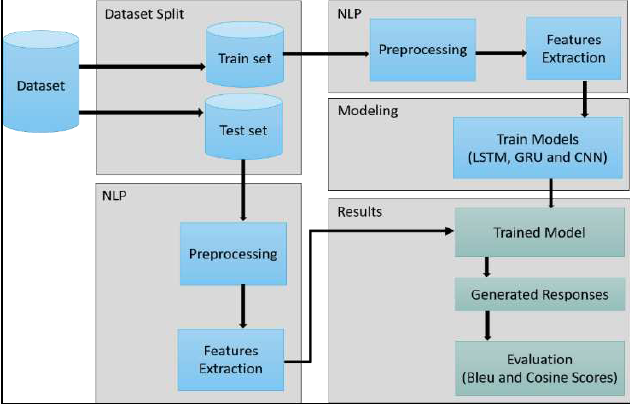
\includegraphics[width=12cm]{architecture.png}
    \caption{Chatbot Architecture}
    \label{fig:architetcture}
\end{figure}
}
\section{Different Approaches }
{\setlength{\baselineskip}{1.1\baselineskip}
%Start writing from here.
Three approaches are studied for implementing natural language processing in chatbot technology:\\
\-\hspace{1.2cm}{\bf {1.\baselineskip} Bidirectional Recurrent Neural Networks} are the most appropriate models for processing sentences , as they have achieved substantial success in text categorization and machine translation.\\
\begin{figure}[htp]
    \centering
    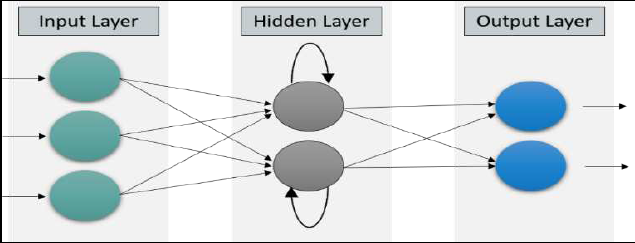
\includegraphics[width=10cm]{brnn.png}
    \caption{Bidirectional RNN Architecture}
    \label{fig:architetcture}
\end{figure} 
\-\hspace{1cm}{\bf {2.\baselineskip} Deep Neural Networks} (DNN) can be defined as RNNs with additional depth , that is , an increased number of hidden layers between the input and the output layers.\\
\begin{figure}[htp]
    \centering
    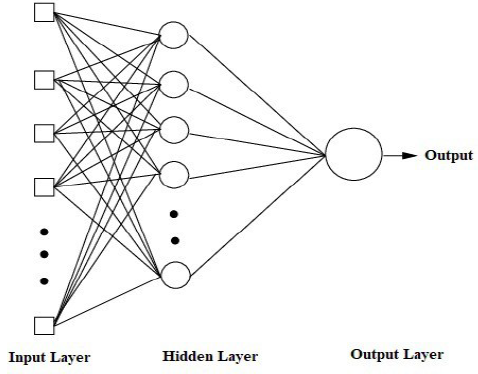
\includegraphics[width=10cm]{dnn.png}
    \caption{DNN Architecture}
    \label{fig:architetcture}
\end{figure}
\-\hspace{1cm}{\bf {3.\baselineskip} Convolutional Neural Networks} (CNN) are chosen mainly for its efficiency, since CNN is faster compared to other text representation and extraction methods.\\
\begin{figure}[htp]
    \centering
    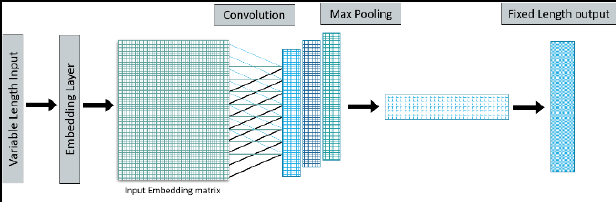
\includegraphics[width=14cm]{cnn.png}
    \caption{CNN Architecture}
    \label{fig:architetcture}
\end{figure}
}
}
\newpage
\section{State-of-the-art Algorithms}
{\setlength{\baselineskip}{1.1\baselineskip}
%Start writing from here.
{\bf Sequence to Sequence Model algorithm} is applied to implement natural language processing in chatbot technology using Bidirectional RNNs. \\
\-\hspace{1cm}Sequence-to-sequence models are used in many fields,
including chat generation, text translation, speech recognition,
and video captioning. The input text enters the encoder network in reverse
order, then it is converted into a sequence of fixed length context vector, which is then used by the decoder to generate the output sequence 
\begin{figure}[h!]
    \centering
    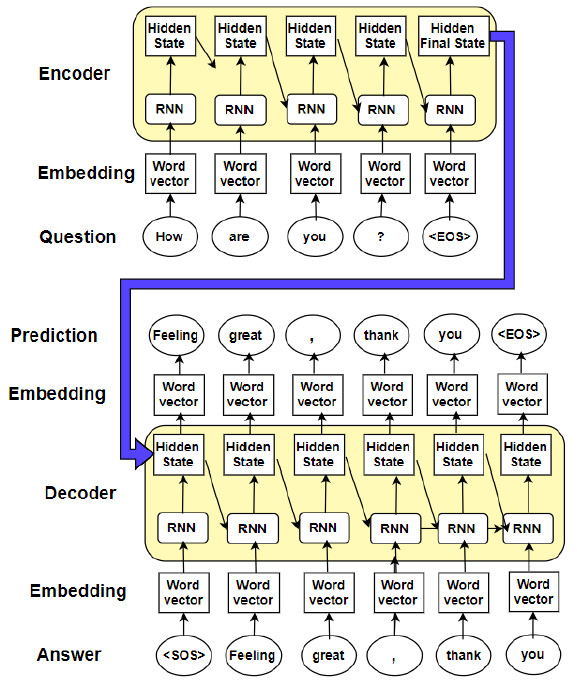
\includegraphics[width=12cm]{seq2seq2.png}
    \caption{Sequence to Sequence Model}
    \label{fig:seq2seq}
\end{figure}
}
\-\hspace{1cm}\\ The following activity happens during the encoding phase:- \\
1) The question string (``How are you ?'') is first tokenized into a list of tokens. A token can be a word or a sub-word of one (1) or more characters and symbols.\\
2) Each token is then associated with a vector which is a subset of input vocabulary.
\newpage
{\large \bf Algorithms} \\  \\ 
{\bf Algorithm 1 : }Training a Sequence to Sequence Model With Attention
Mechanism for Answer Generation \\
{\bf Input:} Question (X)-Answer(Y) pairs, Maximum Answer Tokens to Generate (T), Number of Epochs \\
{\bf Steps :} \\
For epoch 1 to Number of Epochs \\
For the batch of question-answer pairs, X and Y Do \\
1. Encoder: Perform question encoding, generate the hidden states for each timestep \\
2. Decoder: \\
2.1 Generate tokens (with the highest probability) one by one by feeding weighted hidden \\
states from Encoder until maximum answer length is reached, or end of sequence token is generated \\
2.2 Join all tokens to generate an answer (Y') \\
3. Calculate the cross-entropy loss (the difference between Y and Y') \\
4. Update the model parameters \\
End For \\
End For \\
{\bf Output:} Trained Seq2Seq Model \\ \\
{\bf Algorithm 2 : }Sequence to Sequence Model Prediction (Beam Search) \\
{\bf Input:} Trained Seq2Seq Model, Question (Q), Beam Size (k) \\
{\bf Steps :} \\
1. Encoder: Perform question encoding, generate the hidden states for each timestep \\
2. Decoder: \\
2.1 Generate tokens (with probability scores) by feeding weighted hidden states from Encoder \\
2.2 Sort and get the k top tokens based on probability score (this is the hypothesis with 1 word) \\
2.3 Add to beam search list \\
2.4 For each of the hypothesis in the beam search list \\
2.4.1 Generate tokens (with probability scores) by feeding weighted hidden states from Encoder \\
2.4.2 Sort and get the k top tokens \\
2.4.3 Add to the hypothesis in the beam search list \\
2.5 Calculate probabilities for each of the k2 hypothesis, sort and keep only k top hypothesis \\
2.6 Repeat steps 2.4 to 2.5 until maximum answer length is reached or end of sequence token is generated \\
2.7 Sort beam search list and return the hypothesis with the highest probability\\
{\bf Output:} Answer to Question(Q) \\ \\
\section{Discussion}
{\setlength{\baselineskip}{1.1\baselineskip}
%Start writing from here.
Bidirectional Recurrent Neural Networks and Deep Neural Networks are more suitable to implement natural language processing in text-to-text or speech-to-text chat bot technology as compared to Convolutional Neural Networks. \\
\-\hspace{1cm}Comparison between RNN and CNN - 
\begin{center}
\begin{table}[htp]
\label{RNN vs CNN}
\begin{tabular}{|p{8cm}|p{8cm}|}
\cline{1-2}
RNN  & CNN \\
\hline
The conversation is a sequence of words (Can handle arbitrary input and output lengths) & The conversation is a fixed size ( Cannot handle sequential data) \\
\hline
Considers the previously received inputs along with the current input. The LSTM cells used in RNN model allow RNN to memorize previous inputs. & Considers only the current input, and it cannot remember the previous input. \\
\hline
Uses time-series information, hence it is the best suitable model for systems that take the conversation context in its consideration. & Uses connectivity pattern
between its neurons, hence the neurons are arranged in such a way that enables CNN to respond to overlapping regions tiling the visual field. \\
\hline
Used to create a combination of subcomponents (e. g. text generation, language translation) & Used to break a component (e. g. image) into subcomponents (e. g. object in an image) \\
\hline
It is ideal for text and speech generation. & It is ideal for images, videos processing and ranking candidate sentences. \\
\hline
\end{tabular}
\caption{RNN vs CNN}
\end{table}
\end{center}
}

%---------------------------Proposed solution & its Design--------------
\newpage 
\chapter{\centering{Implementation}}
{\setlength{\baselineskip}{1.1\baselineskip}

%---------- Proposed Solution
%those who have done implementation can 
\section{Algorithm/Methodologies}
{\setlength{\baselineskip}{1.1\baselineskip}
%Start writing from here.
Implementation of NLP using Sequence to Sequence Model Algorithm.
\begin{figure}[htp]
    \centering
    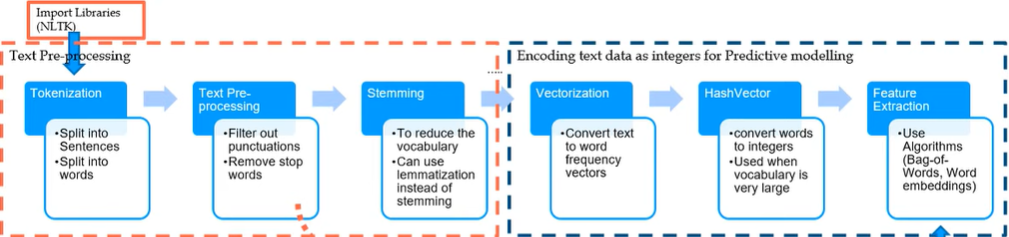
\includegraphics[width=16cm]{nlp steps.png}
    \caption{NLP using Sequence to Sequence Model}
    \label{fig:nlpsteps}
\end{figure} 
}
\section{Proposed Solution}
{\setlength{\baselineskip}{1.1\baselineskip}
%Start writing from here.
Deep Recurrent Neural Networks are the most suitable to implement NLP in chatbot technology. Python code for steps involving Implementation of NLP using sequence to sequence model to create a general purpose chatbot is as follows - \\
{\bf Tokenization} 
\begin{python}
sent_tokens = nltk.sent_tokenize(raw)# converts to list of sentences
word_tokens = nltk.word_tokenize(raw)# converts to list of words
\end{python}
{\bf Lemmatization} 
\begin{python}
# LemTokens will take as input the tokens and return normalized tokens.
def LemTokens(tokens):
   return [lemmer.lemmatize(token) for token in tokens]
\end{python}
{\bf Pre-Processing} 
\begin{python}
remove_punct_dict = dict((ord(punct), None) for punct in string.punctuation)
def LemNormalize(text):
   return LemTokens(nltk.word_tokenize(text.lower().translate(remove_punct_dict)))
\end{python}
{\bf Vectorization} 
\begin{python}
 TfidfVec = TfidfVectorizer(tokenizer=LemNormalize, stop_words='english')
\end{python}
}

\section{Software Requirement Specification}
{\setlength{\baselineskip}{1.1\baselineskip}
%Start writing from here.
}
\subsection{Constraints and Assumptions}
{\setlength{\baselineskip}{1.1\baselineskip}
%Start writing from here.
Dataset used is small, and training it over deep neural networks model leads to over fitting the model, to find the optimal learning rate appropriate precautions must be taken while building the model.
\begin{center}
\begin{table}[htp]
\label{Dataset Description}
\begin{tabular}{|c|p{12cm}|}
\cline{1-2}
Attribute Name  & Description \\
\hline
Tags & Tags are keywords assigned to the patterns and responses for training the chatbot .e.g., "greeting", "bye". \\
\hline
Patterns & These are the types of queries asked by the user to the chatbot. \\
\hline
Responses &  Responses are the answers generated by the chatbot for the respective queries.\\
\hline
Context & Context is given for which the queries require a search and find operation.\\
\hline
\end{tabular}
\caption{Dataset Description}
\end{table}
\end{center}
}
%---------- Design -----------

\subsection{Platform for Implementation and its Specifications}
%Start writing from here.
\begin{itemize}
    \item Latest Python Version 3.9.0 installed on your PC(Windows/Linux).
    \item Jupyter Notebook installed
    \item A software GUI library called 'Tkinter' for Python is used to create a simple user interface.
    \item Libraries Imported :- \\
    \begin{python}
    import nltk # Natural Language ToolKit used for NLP
    import warnings
    import numpy as np
    import random
    import string 
    from sklearn.feature_extraction.text import TfidfVectorizer
    \end{python}
\end{itemize}
\par
\newpage
\section{Result }
%Start writing from here.
{\large \bf Rules-Based Chatbots vs. NLP based Chatbots} \\
\-\hspace{1cm}A rules-based solution “allows brands to deliver experiences to specific segments of people based on the manual creation and manipulation of business rules.” For instance, a brand may set up a chatbot rule that states “If a person mentions the word ‘return,’ have the chatbot reply with our QnA page on how to return a product.” NLP-powered chatbots, on the other hand, analyze past conversation data to “present the most relevant content or experience for each and every visitor in real-time.” It works like this: If a customer has a question about a return because something doesn’t fit, the machine won’t provide a link to a return page because of a rule that has been set up. Instead, the chatbot may provide a specific answer based on past conversations in which similar customers specifically asked about “returns” and “fit.” In short, the main difference comes down to a model’s ability to understand what someone is saying and respond accordingly without help from a human. As specific as a rules-based chatbots can be, they are only as effective as a company’s ability to anticipate every user question and comment. \\ \\
{\large \bf Why NLP based Chatbot is better?} \\
\-\hspace{1cm}Rules-based software can be effective if you want to achieve something you’ve seen work before on a basic level. For example, in the past, anyone who asked us X question expected Y response. ML applications require more data to train, and as a result, can make more informed decisions about what types of behavior may lead to purchase or what types of chatbot answers are most likely to resonate with a customer in real-time.NLP based chatbots make interaction between human and interface more lively.
}
%---------------------------Conclusion ----------------
\newpage 
\chapter{\centering{Applications}}
{\setlength{\baselineskip}{1.1\baselineskip}
\section{State-of-the-art Applications}
%Start writing from here.
\begin{itemize}
    \item Customer Service - The implementation of chatbots in customer service also involves the use of cases of collecting customer feedback.
    \item Media Publishing Applications - Media publishers recognize chatbots as a promising approach for engaging with the audience alongside monitoring the engagement of the audience. As a result, chatbots can help media publishers in obtaining credible and helpful insights regarding audience interests.
    \item Food Ordering - The commonly visible application of chatbots is evident in the case of food delivery. Notable names such as Pizza Hut and KFC use chatbots for allowing customers to place orders through a conversation. 
    \item HealthCare Applications - The chatbot examples in the healthcare sector also showcase the breadth of the reach of chatbots. Chatbots, such as Super Izzy has been helping medical professionals in providing quick medical diagnosis and answers to health-related questions. 
\end{itemize}
\section{Challenges}
\begin{itemize}
    \item Understanding the User Intent - For any Chatbot, the biggest challenge is to understand the user intent and to decode the intent hidden inside the queries and messages.
    \item Building an affordable chatbot solution - Many small and medium enterprises simply skip Chatbots because of the higher cost factor.
    \item Chatbot Testing - As natural language processing (NLP) capability is increasingly getting better, Chatbots are now frequently updated. This is why the testing mechanism should always be used for every update to check the effects of each value addition.
    \item Building a more human chatbot - The last but not the least of all these challenges is building a Chatbot that makes an impression of human conversation to the user on the other end.
\end{itemize}
\par
}

%---------------------------Conclusion ----------------
\newpage 
\chapter{\centering{Conclusion and Future Scope}}
{\setlength{\baselineskip}{1.1\baselineskip}
%Start writing from here.
\-\hspace{1cm}This study involves the application of Natural Language Processing to create chatbot technology using Artificial Neural Networks.To explore Most suitable approach of implementing Natural Language Processing in chatbots. According to the results, Deep Recurrent Neural Networks are most suitable for creating a chatbot based on Natural Language Processing using Sequence-to-Sequence Model Algorithm.

Implementation of Natural Language Processing in chatbot was planned by implementing Natural Language Processing steps involved ,to import Natural Language ToolKit in Python and implement sequence-to-sequence algorithm for creating a chatbot and its working Tkinter GUI.A very basic chatbot was built using a small Kaggle dataset , all the Natural Language Processing steps are implemented by importing Natural Language ToolKit. To check whether the chatbot is working efficiently using Machine Learning model on Tkinter GUI is not implemented.

\par

}
\end{normalsize}



%---------------------------References----------------
\newpage
\addcontentsline{toc}{chapter}{References}
\bibliographystyle{plain}
\begin{normalsize}
				{\setlength{\baselineskip}{1.1\baselineskip}
{
\begin{thebibliography}{9}

\bibitem{a} G Krishna Vamsi , Akhtar Rasool , Gaurav Hajela A Deep Neural Network Based Human to Machine Conversation Model , IEEE 11th ICCCNT 2020
July 1-3, 2020 - IIT - Kharagpur 
\bibitem{b} %Start writing from here.
Ramakrishna Kumar, Maha Mahmoud Ali(2020) A Review on Chatbot Design and Implementation Techniques, National University of Science and Technology, Muscat, Oman , Feb 2020.
\bibitem{c} Moneerh Aleedy, Hadil Shaiba, Marija Bezbradica (2019) Generating and Analyzing Chatbot Responses using Natural Language Processing,International Journal of Advanced Computer Science and Applications
\bibitem{d} KULOTHUNKAN PALASUNDRAM,NURFADHLINA MOHD SHAREF, KHAIRUL AZHAR KASMIRAN,AND AZREEN AZMAN Enhancements to the Sequence-to-Sequence-Based Natural Answer Generation Models,Intelligent Computing Research Group, Faculty of Computer Science and Information Technology, Universiti Putra Malaysia, IEEE Access,February 24, 2020.



\end{thebibliography}
\par}
}

\newpage					%start a new page

\appendix
\addcontentsline{toc}{chapter}{Plagiarism Report}

% Required package


    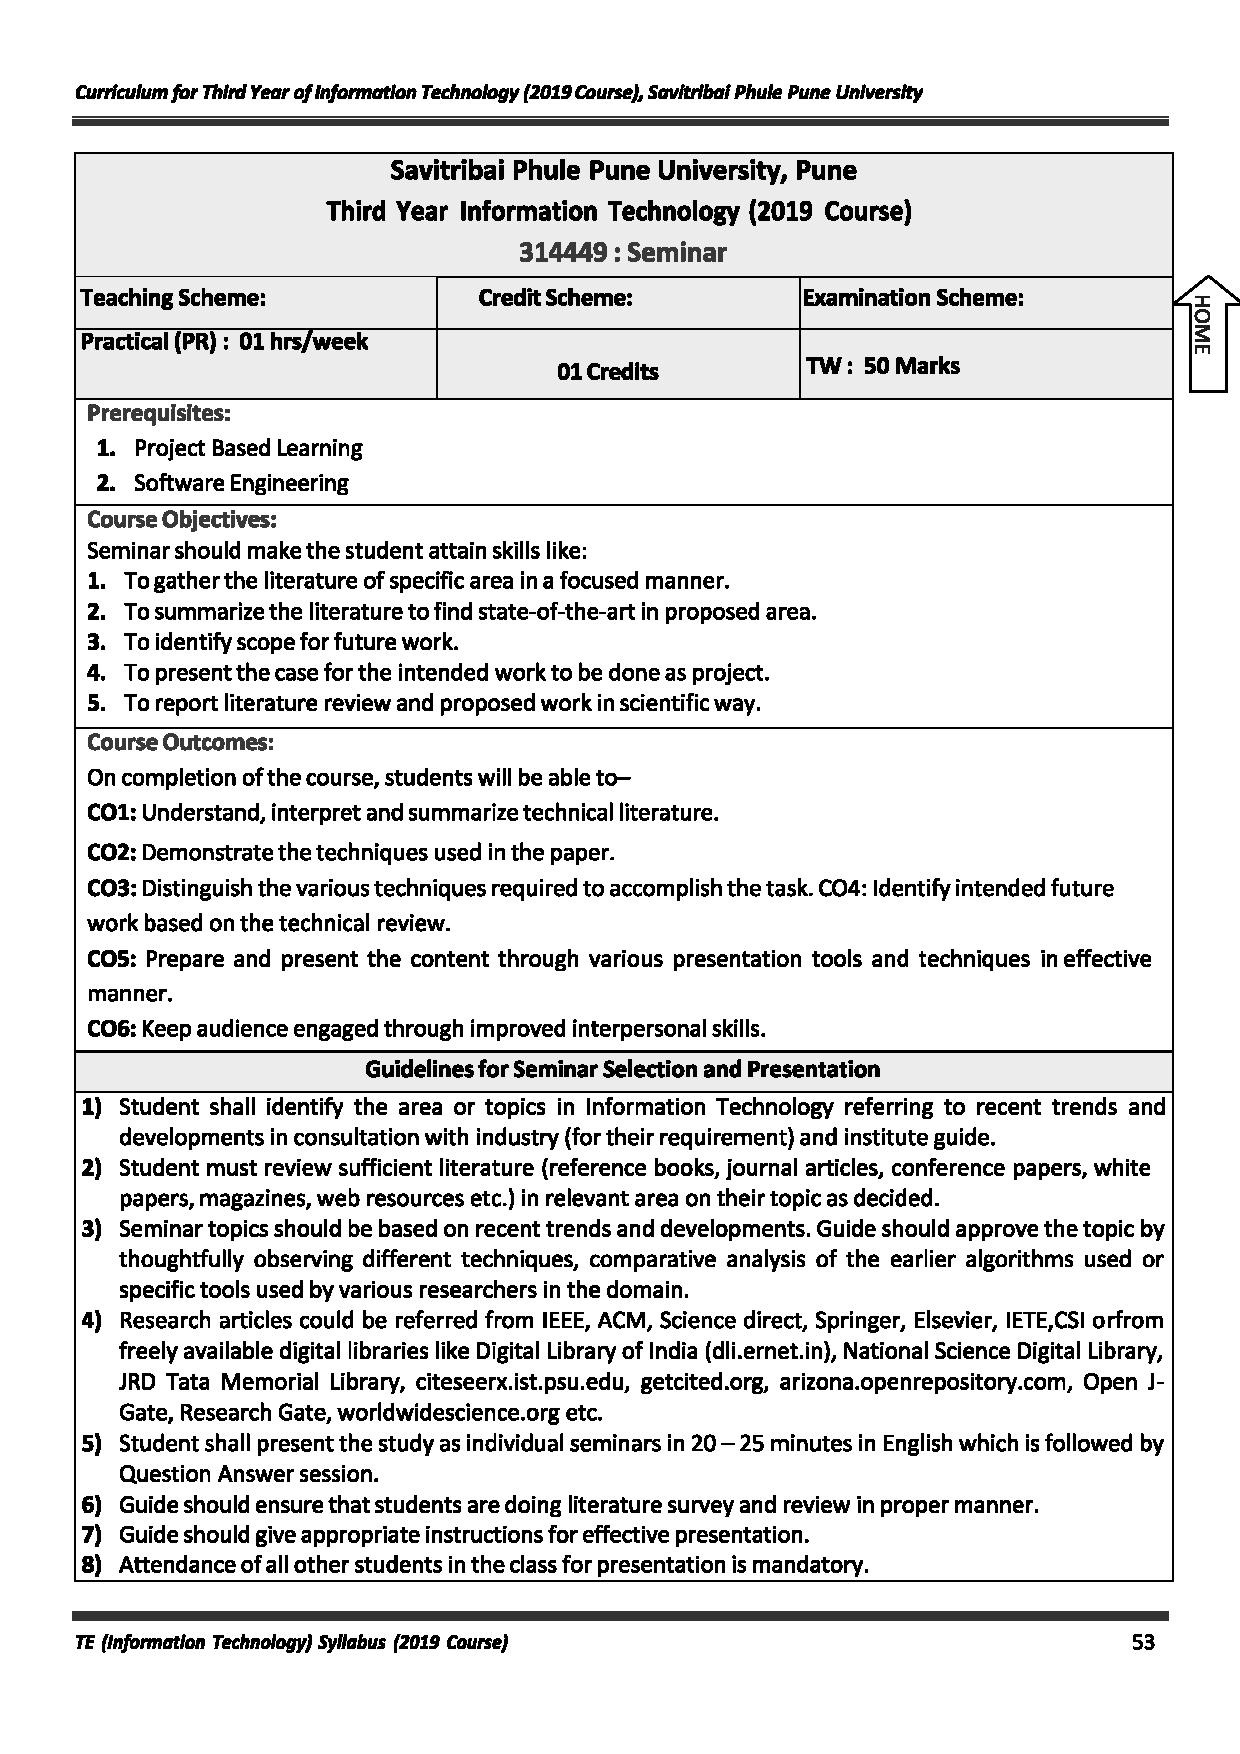
\includepdf[page={1,2,3}]{Seminar.pdf} 
    % Uplaod plagarism Report file in this project first  and now include Plagiarism report %file in PDF Format.
   % here instead of Seminar.pdf,write the name of plagarism report file.
   % For Example Here in this project Seminar.pdf file has been added.
   
\end{normalsize}
\end{document}
